\documentclass[../Assignment-3-LPSMT.tex]{subfiles}
\graphicspath{{\subfix{../img/}}}

\begin{document}

\chapter{Architettura}

\begin{center}
  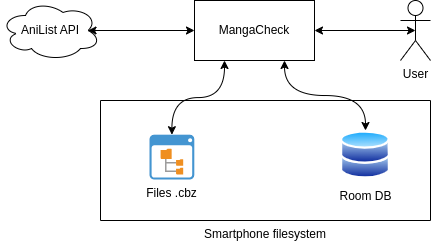
\includegraphics[scale=0.6]{architettura2.png}
\end{center}

\section{Room DB}

L'applicazione crea un database \href{https://www.sqlite.org/index.html}{SQLite} in locale, la comunicazione con esso avverrà attraverso \href{https://developer.android.com/reference/androidx/room/package-summary}{Room}.\\
Il DB sarà composto da 2 tabelle:
\begin{enumerate}
  \item \textbf{Chapters}: contenente tutti i capitoli aggiunti all'applicazione, sono memorizzati tutti i dati fondamentali per risalire al file e all'opera di appartenenza.\\
  \item \textbf{Series}: è l'insieme di tutte le serie che sono state aggiunte all'applicazione, vi sono memorizzate anche informazioni ottenute dalle API di \href{https://anilist.gitbook.io/anilist-apiv2-docs/}{AniList}.
\end{enumerate}

\section{Files .cbz}

Attraverso un \texttt{Intent} l'applicazione può aprire il file explorer di default e tramite quello selezionare un file che rispetta il MIME type~\cite{rfc6838} \texttt{application/x-cbz}.\\
Il file non verrà spostato nello spazio privato per evitare sprechi di memoria, verrà quindi salvato solo L'URI del file selezionato.

\section{AniList API}

\'E stata rimossa qualsiasi forma di intermediazione tra applicazione e le API di AniList.\\
Per interfacciarsi con il server abbiamo utilizzato il client GraphQL \href{https://www.apollographql.com/docs/kotlin}{Apollo} che ci ha permesso di creare query direttamente dal dispositivo.\\
L'eliminazione di un layer intermedio ci ha permesso di gestire al meglio le risorse che ottenevamo, come le immagini grazie a \href{https://bumptech.github.io/glide/}{Glide}.

% \section{DB remoto}

% Il database remoto è stato scritto in \href{https://www.sqlite.org/index.html}{SQLite} e viene gestito da un server \href{https://flask.palletsprojects.com/en/2.3.x/}{Flask}, il contenuto del Database è stato ottenuto sfruttando le API di \href{https://anilist.gitbook.io/anilist-apiv2-docs/}{AniList}.\\
% Nel database abbiamo messo le principali informazioni di ogni manga: un id, il titolo, descrizione, immagini di copertina, capitoli, volumi e stato di pubblicazione.\\
% Per effettuare richieste alle API del server Flask abbiamo optato per l'utilizzo della libreria \href{https://ktor.io/}{Ktor} dato il grande di team che la sviluppa essendo gestita da JetBrains.\\
% Le richieste al server sono state gestite in modo asincrono rispetto al thread principale, e i loro risultati sono stati processati con delle classi helper per formattare in modo corretto i dati ricevuti.\\

% \section{File nello spazio privato}

% L'applicazione crea dei file nel proprio spazio privato per poter gestire tutti i dati dell'utente.\\
% I file più importanti sono due \emph{xml} che fungono da elenco delle varie library e reading che un utente possiede, per scrivere e leggere su queste liste abbiamo usato delle coroutine per cercare di rendere l'applicazione più responsive possibile.\\
% Per cercare di massimizzare l'efficienza delle richieste alle API del server abbiamo deciso di fare il caching delle immagini di copertina dei vari manga che vengono richiesti, questo ci permette di fare la richiesta per un'immagine solo se nella cartella di cache facciamo una miss del dato.\\
% Per la gestione dei capitoli abbiamo deciso di creare, per ogni library, una cartella chiamata come l'id dell'opera stessa e di inserirci i capitoli che un utente carica, la nomenclatura dei capitoli è la seguente \emph{<numero\_capitolo>.cbz}.

% \begin{center}
%   \lstinputlisting[style=xml, caption=Esempio del file readingList.xml]{./snippet-codice/readingList.xml}
%   \lstinputlisting[style=xml, caption=Esempio del file libraryList.xml]{./snippet-codice/libraryList.xml}
% \end{center}

% \section{File nel resto del device}

% Manga-check avrà anche accesso allo storage esterno del device, questo permetterà di poter importare/esportare la propria \emph{reading list}, verrà mostrato un messaggio Toast se la lista non esiste ancora e si trenta di esportarla, mentre non verrà renderizzata la schermata se il file importato dovesse essere malformato.
% I vari capitoli verranno importati dallo storage estrerno all'app e copiati in quello privato come sopra descritto.\\
% Sia per gli \emph{xml} che per i \emph{cbz} la selezione è stata forzata ai MIME type~\cite{rfc6838} dei rispettivi tipi di file.

\end{document}
